\section{Abzählbare Mengen}
Eine Menge \(A\) heisst \emph{abzählbar}, wenn \(A=\varnothing\) oder eine der folgenden (äquivalenten) Bedingungen erfüllt ist:
\begin{itemize}
  \item \(|A|\le | \mathbb{N} |\)
  \item Es existiert eine surjektive Funktion \(f:\mathbb{N}\twoheadrightarrow A\).
  \item Es existiert eine injektive Funktion \(f:A\hookrightarrow\mathbb{N}\).
\end{itemize}
\emph{Bemerkung:} Ist \(A\) abzählbar und unendlich, so gilt \(|A|=|\mathbb{N}|\).

\subsection{Beispiele}
\begin{itemize}
  \item Die leere Menge \(\varnothing\) ist abzählbar.
  \item Jede Teilmenge \(A\subseteq\mathbb{N}\) ist abzählbar (insbesondere \(\mathbb{N}\) selbst).
  \item \(\mathbb{Z}\) ist abzählbar.
  \item \(\mathbb{Q}\) ist abzählbar (als Schlussfolgerung aus Abzählbarkeit von \(\mathbb{Z}\times\mathbb{Z}\) und Quotientenbildung).
\end{itemize}

\subsection{Wichtige Aussagen}
\begin{itemize}
  \item Jede endliche Menge ist abzählbar. (Beweis: Aufzählung der Elemente liefert eine surjektive Abbildung \(\mathbb{N}\twoheadrightarrow A\).)
  \item Jede Teilmenge einer abzählbaren Menge ist abzählbar. (Bild- bzw. Einschränkungsargument.)
  \item Bild einer abzählbaren Menge unter einer surjektiven Abbildung ist abzählbar. (Komposition surjektiver Abbildungen.)
  \item \(\mathbb{N}\times\mathbb{N}\) ist abzählbar. Daraus folgt die Abzählbarkeit von \(\mathbb{Z}\times\mathbb{Z}\) und damit \(\mathbb{Q}\).\\
  \begin{center}
    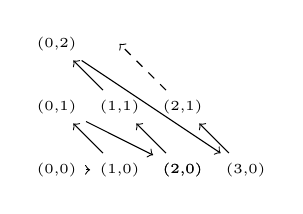
\begin{tikzpicture}[scale=.8]
    \node (0-0) at (0, 0) {\tiny (0,0)};
    \node (1-0) at (1, 0) {\tiny (1,0)};
    \node (2-0) at (2, 0) {\tiny (2,0)};
    \node (3-0) at (3, 0) {\tiny (3,0)};
    \node (0-1) at (0, 1) {\tiny (0,1)};
    \node (1-1) at (1, 1) {\tiny (1,1)};
    \node (2-1) at (2, 1) {\tiny (2,1)};
    \node (2-0) at (2, 0) {\tiny (2,0)};
    \node (0-2) at (0, 2) {\tiny (0,2)};
    \draw[->] (0-0) -- (1-0);
    \draw[->] (1-0) -- (0-1);
    \draw[->] (0-1) -- (2-0);
    \draw[->] (2-0) -- (1-1);
    \draw[->] (1-1) -- (0-2);
    \draw[->] (0-2) -- (3-0);
    \draw[->] (3-0) -- (2-1);
    \draw[->, dashed] (2-1) -- (1,2);
  \end{tikzpicture}
  \end{center}
  \item Jede abzählbare Vereinigung abzählbarer Mengen \(\bigcup_{i\in\mathbb{N}} A_i\) ist abzählbar. (Beweisidee: doppelte Indizierung und Aufzählung aller Paare \((i,n)\).)
\end{itemize}
